\newpage
\section{Análisis de Componentes Principales}
\subsection{Enunciado}
Aplicación del PCA: Utilizando Python y las librerías correspondientes (sklearn, pandas, matplotlib, etc.), aplicarán PCA sobre los datos estandarizados.

Análisis 1: Elección de Componentes Principales: Deberán determinar el número 
adecuado de componentes a retener basándose en la varianza explicada acumulada. 
Como pauta: retener los componentes principales que expliquen al menos el 80 por ciento
de la varianza total. Esto suele dar un buen balance entre simplificación y retención 
de la información clave. En este punto se quedara con un número determinado de componentes según el criterio de la varianza total.

Análisis 2: Gráfica Unitaria y Bautizo de Ejes:
Una vez seleccionados los dos primeros componentes, generar una gráfica de dispersión 
(scatter plot) en dos dimensiones con los datos proyectados en el espacio definido por 
los primeros dos componentes principales. Interpretar qué representa cada eje en 
función de las variables originales. Basado en las cargas de las variables en cada componente, asignar nombres descriptivos a los ejes (por ejemplo, “Eficiencia Operacional” o “Costo de Producción”). En este punto se quedara con 2 componentes.

\subsection{Aplicación del PCA}
Utilizando los datos estandarizados, se procede a aplicar PCA.

\begin{verbatim}
scaler = StandardScaler()
X_scaled = scaler.fit_transform(X)
pca = PCA(n_components=2) 
X_pca = pca.fit_transform(X_scaled)
\end{verbatim}


\subsection{Análisis 1: Elección de Componentes Principales}
\subsubsection{PCA con 2 componentes}
Tomando en cuenta que para este análisis se utilizarán los dos primeros componentes, 
con la gráfica y también se procede a calcular la varianza explicada acumulada.

\begin{figure}[h!]
    \centering
    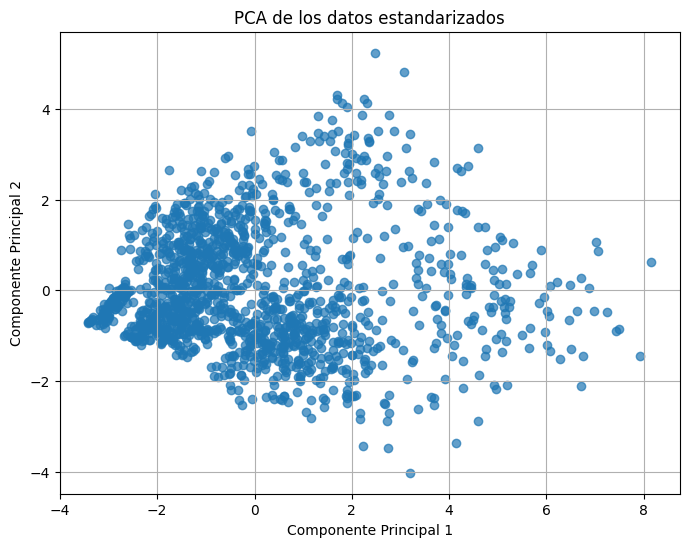
\includegraphics[width=1\textwidth]{images/pca-2-components.png}
    \caption{PCA con los dos primeros componentes}
    \label{fig:pca_2_components}
\end{figure}

Los resultados de la varianza nos muestran que:    
\begin{itemize}
    \item \textbf{Varianza explicada por cada componente:} [0.51429629, 0.19511065]
    \begin{itemize}
        \item El primer componente explica el 51.43\% de la varianza.
        \item El segundo componente explica el 19.51\% de la varianza.
    \end{itemize}

    \item \textbf{Varianza acumulada:} [0.51429629, 0.70940693]
    \begin{itemize}
        \item La suma acumulada de los dos primeros componentes es aproximadamente 71.94\%.
    \end{itemize}
\end{itemize}

Esto nos muestra que los dos primeros componentes explican aproximadamente el 71.94\% de la varianza total, 
pero no son lo suficientemente altos como para retenerlos, por lo cual vamos a probar con 3 componentes.

\subsubsection{PCA con 3 componentes}
Tomando en cuenta que para este análisis se utilizarán los tres primeros componentes.

\begin{verbatim}
pca = PCA(n_components=3) 
X_pca = pca.fit_transform(X_scaled)
\end{verbatim}

Al ser tres componentes, se procede a graficar en 3 dimensiones.

\begin{figure}[H]
    \centering
    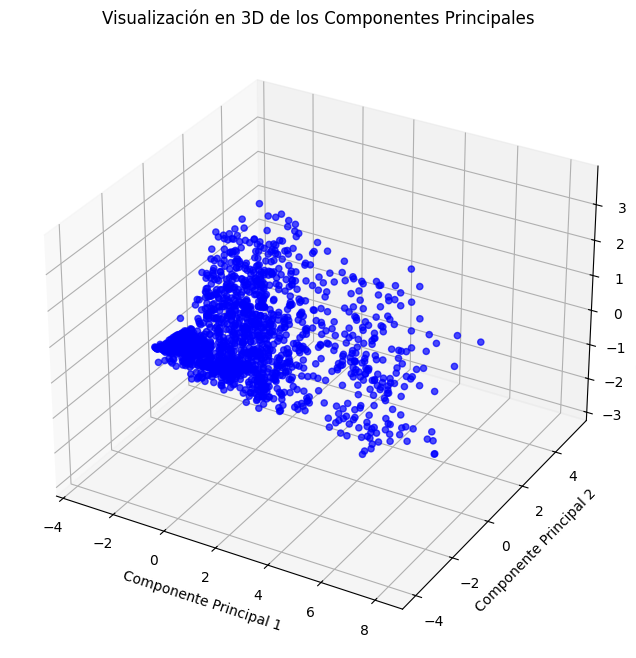
\includegraphics[width=1\textwidth]{images/pca-3-components.png}
    \caption{PCA con los tres primeros componentes}
    \label{fig:pca_3_components}
\end{figure}

Los resultados de la varianza nos muestran que:    
\begin{itemize}
    \item \textbf{Varianza explicada por cada componente:} [0.51429629, 0.19511065, 0.09318736]
    \begin{itemize}
        \item El primer componente explica el 51.43\% de la varianza.
        \item El segundo componente explica el 19.51\% de la varianza.
        \item El tercer componente explica el 9.32\% de la varianza.
    \end{itemize}

    \item \textbf{Varianza acumulada:} [0.51429629 0.70940693 0.80259429]
    \begin{itemize}
        \item La suma acumulada de los dos primeros componentes es aproximadamente 80.26\%.
    \end{itemize}
\end{itemize}

Esto nos muestra que los tres primeros componentes explican aproximadamente el 80.25\% de la varianza total,
y que ellos capturan la mayoría de la información relevante de los datos principales


\subsection{Análisis 2: Gráfica Unitaria y Bautizo de Ejes}

Veremos las cargas de las variables de los 3 componentes
\begin{table}[h!]
\centering
\begin{tabular}{|l|r|r|r|}
\hline
\textbf{Variable} & \textbf{PC1} & \textbf{PC2} & \textbf{PC3} \\ \hline
Age                       & 0.275081  & 0.383681   & 0.156552  \\ \hline
JobLevel                  & 0.383995  & 0.264553   & -0.367414 \\ \hline
MonthlyIncome             & 0.376033  & 0.279349   & -0.380146 \\ \hline
NumCompaniesWorked        & 0.045272  & 0.486488   & 0.747841  \\ \hline
TotalWorkingYears         & 0.404073  & 0.242809   & -0.027500 \\ \hline
YearsAtCompany            & 0.394229  & -0.283142  & 0.042967  \\ \hline
YearsInCurrentRole        & 0.338323  & -0.353622  & 0.198766  \\ \hline
YearsSinceLastPromotion   & 0.299302  & -0.266479  & 0.252375  \\ \hline
YearsWithCurrManager      & 0.332705  & -0.364568  & 0.175835  \\ \hline
\end{tabular}
\caption{Cargas de cada variable en los componentes principales}
\end{table}

Observemos las cargas de cada variable en los tres primeros componentes principales (PC1, PC2, y PC3) para entender cómo contribuyen las variables originales a cada componente:

\subsubsection*{Componente Principal 1 (PC1)}
Las cargas más altas en PC1 son:
\begin{itemize}
    \item TotalWorkingYears (0.404073)
    \item YearsAtCompany (0.394229)
    \item JobLevel (0.383995)
    \item MonthlyIncome (0.376033)
    \item Age (0.275081)
\end{itemize}

\textbf{Interpretación:} Este componente parece estar fuertemente asociado con la experiencia laboral acumulada y el nivel de ingreso, lo que sugiere que podría interpretarse como \textbf{"Experiencia y Nivel de Ingreso"}.

\subsubsection*{Componente Principal 2 (PC2)}
Las cargas más altas en PC2 son:
\begin{itemize}
    \item NumCompaniesWorked (0.486488)
    \item Age (0.383681)
    \item YearsWithCurrManager (-0.364568)
    \item YearsInCurrentRole (-0.353622)
    \item JobLevel (0.264553)
\end{itemize}

\textbf{Interpretación:} Este componente parece estar relacionado con la movilidad laboral y factores de estabilidad en el rol. El hecho de que tenga cargas positivas en \textit{NumCompaniesWorked} y \textit{Age}, junto con cargas negativas en \textit{YearsWithCurrManager} y \textit{YearsInCurrentRole}, sugiere una relación entre la estabilidad laboral y la experiencia con el actual jefe. Podemos llamarlo \textbf{"Estabilidad y Movilidad Laboral"}.

\subsubsection*{Componente Principal 3 (PC3)}
Las cargas más altas en PC3 son:
\begin{itemize}
    \item NumCompaniesWorked (0.747841)
    \item MonthlyIncome (-0.380146)
    \item JobLevel (-0.367414)
\end{itemize}

\textbf{Interpretación:} PC3 parece representar una contraposición entre movilidad laboral e ingresos. La alta carga en \textit{NumCompaniesWorked} junto con las cargas negativas en \textit{MonthlyIncome} y \textit{JobLevel} indican una posible relación inversa entre la movilidad y los ingresos. Este componente podría llamarse \textbf{"Movilidad versus Ingreso"}.

Tomando en cuenta el renombre de los componentes, la gráfica es la siguiente, 
pero aclarando que eje Z es Movilidad versus Ingreso:

\begin{figure}[H]
    \centering
    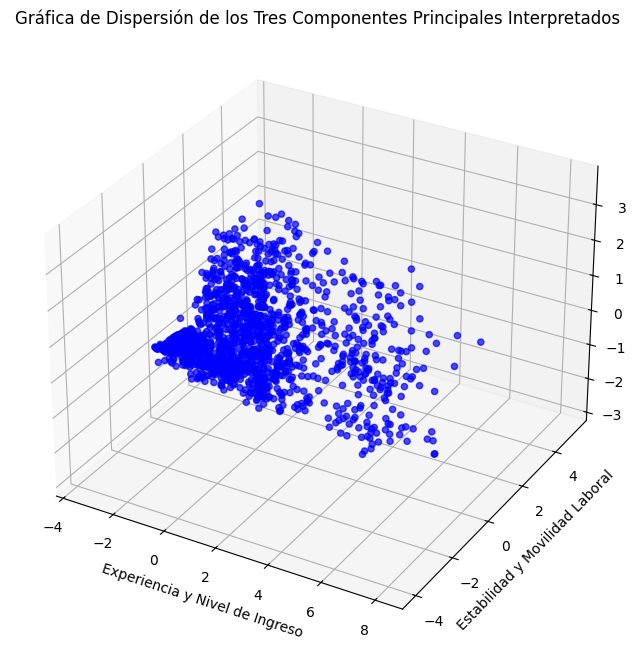
\includegraphics[width=1\textwidth]{images/pca-3-renamed.png}
    \caption{PCA con los tres primeros componentes renombrados}
    \label{fig:pca_3_components_renamed}
\end{figure}